%%%Correct the file name.
%X: book number
%Y: part number
%ZZZ: page number in three digits. So page 3 would be 003.

\documentclass[11pt]{amsbook}

\usepackage{../HBSuerDemir}	% ------------------------


\begin{document}

% ++++++++++++++++++++++++++++++++++++++
\hPage{b1p1/15}
% ++++++++++++++++++++++++++++++++++++++
will be treated in Chapter.\\

We conclude this section by two classification of numbers:\\\\



% =======================================







% =======================================





% =======================================


%\begin{figure}[htb]
%	\centering
	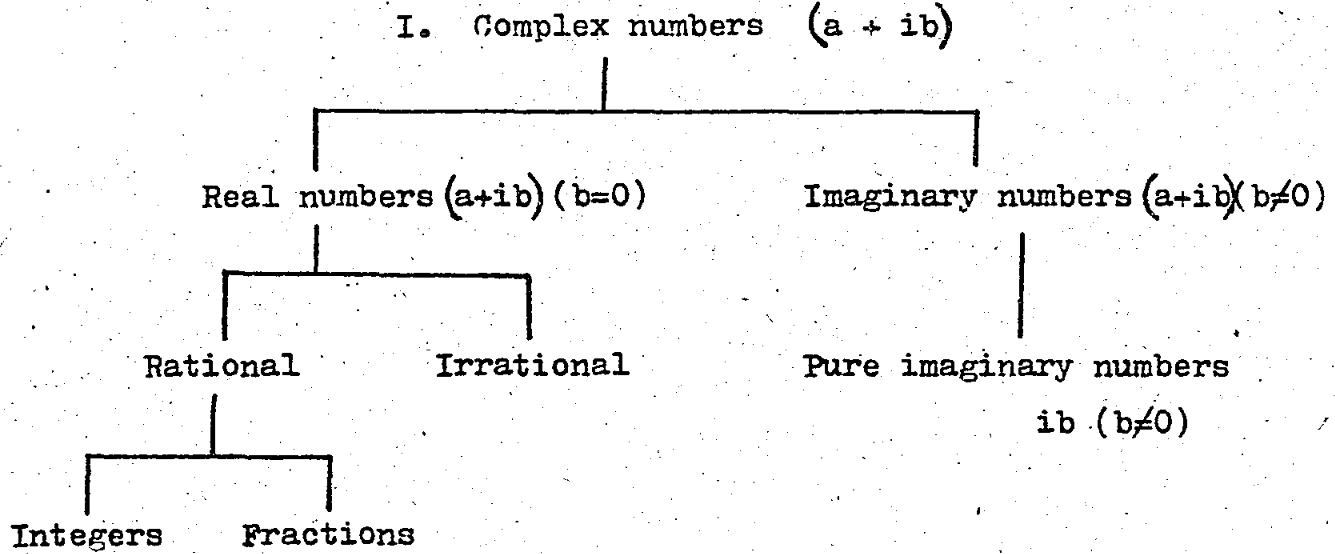
\includegraphics[width=1\textwidth]{images/b1p1-015-fig01}
%	\caption{Classification of complex numbers}
%	\label{fig:classificationOfComplexNumbersA}
%\end{figure}

%\begin{figure}[htb]
%	\centering
	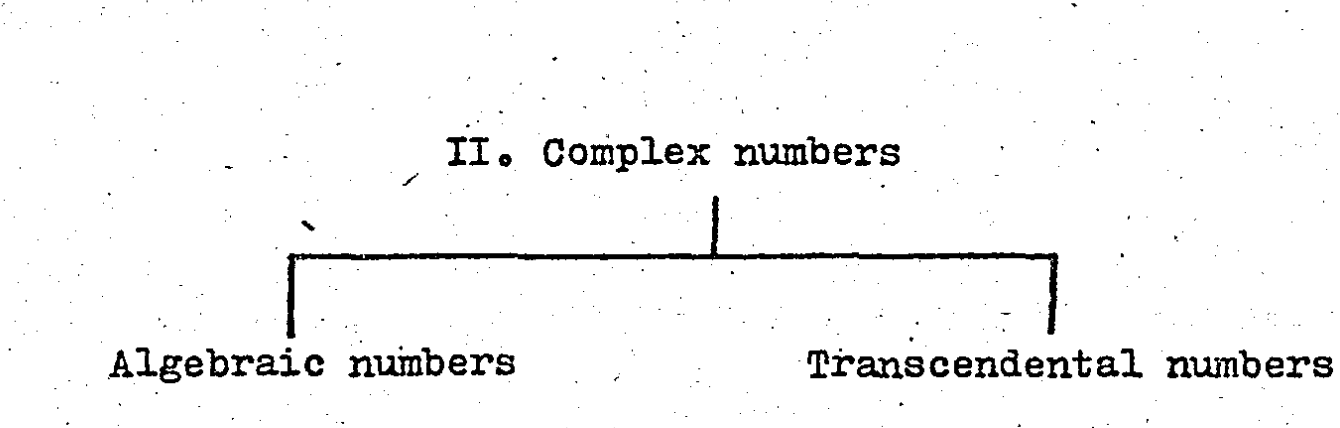
\includegraphics[width=1\textwidth]{images/b1p1-015-fig02}\\
%	\caption{Classification of complex numbers}
%	\label{fig:classificationOfComplexNumbersA}
%\end{figure}

\subsection{EXERCISES}
\paragraph{}

\paragraph{\hspace{0.5cm}1. Construct the following numbers on the number axis:}

\paragraph{\hspace{1.5cm}a) $3/5$\hspace{2.6cm}	b) $-7/3$\hspace{0.6cm} \emph{(use Thales Theorem)}}

\paragraph{\hspace{1.5cm}c) $\sqrt{8}$\hspace{2.8cm}	d) $\sqrt{12}$ \hspace{0.8cm}\emph{(use Pythagorean Theorem)}}

\paragraph{}
\paragraph{\hspace{0.5cm}2. Give examples of two irrational numbers such that their}




% =======================================================
\end{document}  

%==== templates ====

%==== environments ====

%\begin{figure}[htb]
%	\centering
%	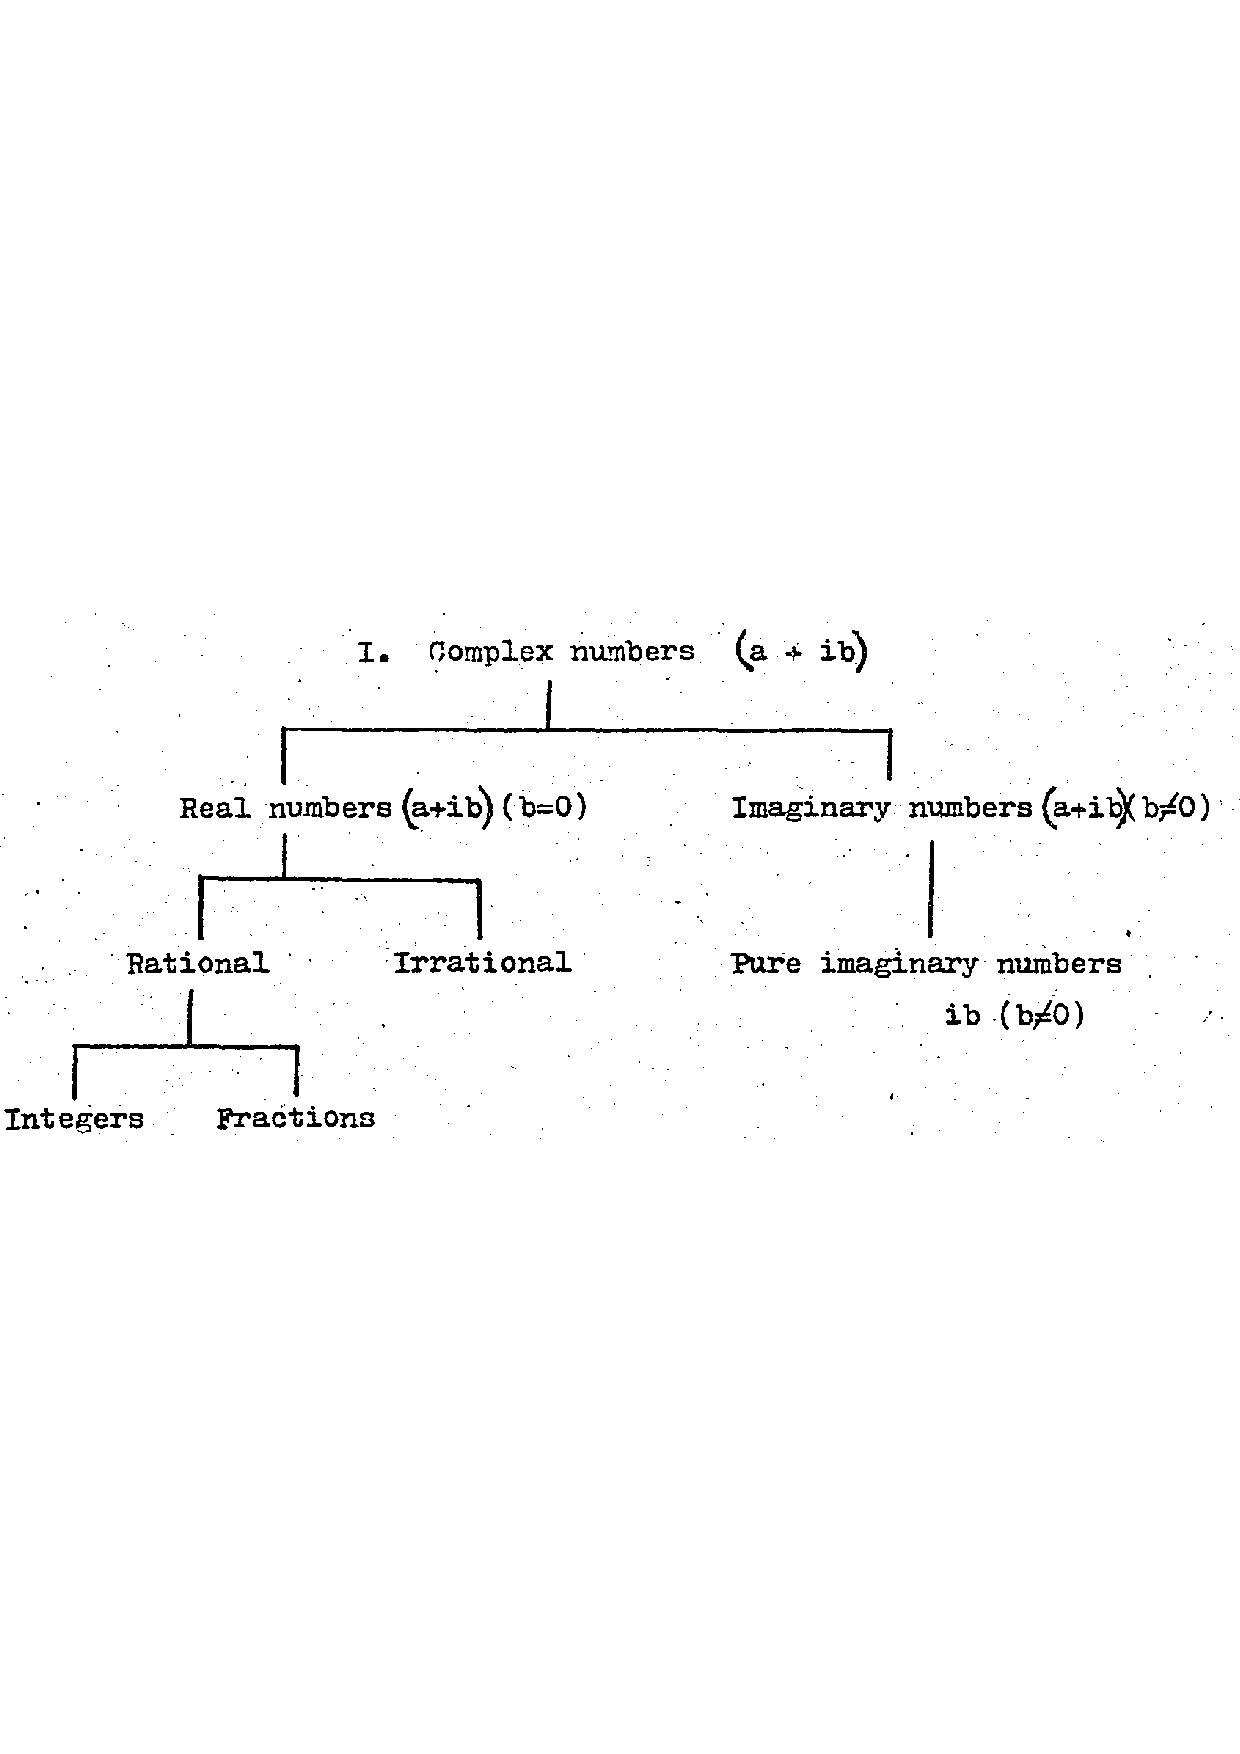
\includegraphics[width=0.9\textwidth]{images/SD-1-1p15A}
%	\caption{Classification of complex numbers}
%	\label{fig:classificationOfComplexNumbersA}
%\end{figure}

%\begin{center}
%\begin{tabular}{cc}
%\end{tabular}
%\end{center}

%\begin{exmp}
%\begin{hSolution}
%\end{hSolution}
%\end{exmp}

%\begin{hEnumerateAlpha}
%\end{hEnumerateAlpha}

%\begin{hEnumerateRoman}
%\end{hEnumerateRoman}

%$
%\begin{bmatrix}
%\end{bmatrix}
%$

%\frac{aaaa}{bbb}
%\frac{a_{n}}{b_{n}}
%\left( aaaa \right)
%\Longrightarrow

%\begin{multicols}{2}
%	bb
%\columnbreak
%	aa
%\end{multicols}
